\chapter{Der Integralsatz von Gauß}

(Einleitung siehe Aufschrieb)

\begin{theorem}
  Für $\Omega \subseteq \mathbb{R}^n$ offen sind äquivalent:
  \begin{enumerate}
    \item Plättung:\\
      $\forall \ p \in \partial \Omega \ \exists \ W \subseteq \mathbb{R}^n$ offen mit $p \in W$ und $\Phi: W\to \Phi(W)$\\
      $C^1$-Diffeomorphismus mit:
      $$\Phi(W \cap \Omega) = \mathbb{H}^n \cap \Phi(W) \text{ wobei } \mathbb{H}^n = \mathbb{R}^{n-1} \times (-\infty, 0)$$
      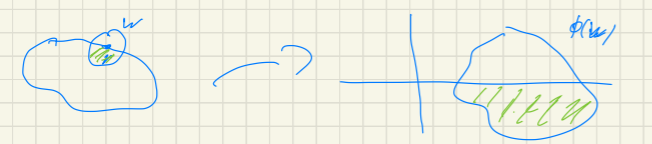
\includegraphics[width=.8\textwidth]{img/IX_1_Plaettung.png}
    \item Subniveau:\\
      $\forall p\in \partial \Omega \ \exists W \subset \mathbb{R}^n$ offen mit $p \in W$ und $h \in C^1(W)$ mit $Dh(q) \neq 0) \\\forall q \in W$, sodass $\Omega \cap W = \{q \in W \ | \ h(q) < 0\}$
    \item Subgraph:\\
      $\forall p \in \partial\Omega \ \exists \script{U} \subseteq \mathbb{R}^{n-1}$ offen $\exists$ offenes Intervall $I \subseteq \mathbb{R} \ \exists C^1$-Funktion $u: \script{U} \to I$, sodass nach geeigneter Umnummerierung der Koordinaten gilt:
      $$\Omega \cap (\script{U} \times I) = \{(x,y) \in \script{U} \times I \ | \ y < u(x)\}$$
  \end{enumerate}
  Die Menge $\Omega$ hat $C^1$-Rand wenn eines (und damit jedes) der drei Kriterien erfüllt ist.
\end{theorem}
\begin{proof}
  siehe Blatt 12
\end{proof}

\begin{lemma}
  In der Situation von Satz IX.1,3) gilt:
  \begin{align*}
    \partial \Omega \cap(\script{U}\times I) &= \{(x,y) \in \script{U} \times I \ | \ y = u(x)\}\\
    (\mathbb{R}\setminus \bar{\Omega}) \cap (\script{U}\times I) &= \{(x,y) \in \mathbb{U} \times I \ | \ y > u(x)\}
  \end{align*}
  $\implies \partial \Omega$ ist $(n-1)$-dimensionale $C^1$-Untermannigfaltigkeit des $\mathbb{R}^n$ nach dem Graphenkriterium bei Untermannigfaltigkeiten.
\end{lemma}
\begin{proof}
  Mit $h: \script{U} \times I \to \mathbb{R}$, $h(x,y) = y-u(x)$ \\
  Vor. $\implies \Omega \cap (\script{U}\times I) = \{ h<0 \}$ \\
  $h$ stetig $\implies \partial \Omega \cap (\script{U}\times I) \subset \{ h=0\}$ \\
  Ist $h(x,y) = 0$ so folgt für $\epsilon$ klein $(x,y-\epsilon)\in\script{U}\times I$ und $h(x,y-\epsilon) = h(x,y) - \epsilon < 0 \rightarrow (x,y-\epsilon)\in\Omega \cap (\script{U}\times I)\\
  \implies (x,y) \in \bar{\Omega}$ und wegen $(x,y) \notin \Omega \implies (x,y) \in \partial\Omega \cap (\script{U}\times I) \implies \partial\Omega \cap (\script{U}\times I) = \{ h=0\}$ \\
  Zweite Aussage folgt aus $\bar{\Omega} = \Omega \cup \partial\Omega$
\end{proof}

\sidenote{Vorlesung 24}{05.02.2021}
\begin{lemma}
  $\Omega \subseteq \mathbb{R}^n$ offen mit $C^1$-Rand. Dann gibt es zu $p \in \partial\Omega$ genau einen Vektor $\nu(p)\in \mathbb{R}^n$ mit
  \begin{enumerate}
    \item $\nu(p) \perp T_p(\partial \Omega)$ und $||\nu(p)|| = 1$
    \item $p + t \nu(p) \notin \Omega$ für $t$ hinreichend klein
  \end{enumerate}
  $\nu:\partial\Omega\to\mathbb{R}^n, n \mapsto \nu(p)$ ist stetig und heißt \textbf{äußere Normale} von $\Omega$.
\end{lemma}

\begin{remark}[Erinnerung: Tangentialraum]
  $\nu \in \mathbb{R}^n$ heißt \textbf{Tangentialvektor} von $M \subseteq R^n, C^1$-Untermannigfaltigkeit in $p\in M$, falls $\gamma:(-\delta, \delta) \to M$ existiert mit $\gamma(0) = p, \gamma'(0) = \nu$\\
  $T_pM = \{$Alle Tangentualvektoren$\}$ $(n-1)$-dimensionaler Untervektorraum.
\end{remark}

\begin{proof}
  Wähle mit Satz IX.1,3) nach ? Umnummerierung der Koordinaten $\Omega \cap (\script{U}\times I) = \{ (x,y)\in \script{U}\times I: y < u(x) \}$ \\
  Sei $q\in \partial\Omega \cap (\script{U}\times I)$ \\
  Lemma IX.2 $\implies f:\script{U} \to \mathbb{R}^n$, $f(x) = (x, u(x))$ ist lokale Para. von $\partial\Omega$ \\
  $T_q(\partial\Omega)$ in $q = (x, u(x))$ hat Basis $(e_i, \frac{\partial u}{\partial x_i}(x)) = \frac{d}{dt} f(x+te_i)|_{t=0}$ für $i=1, ..,n-1$\\
  Definiere auf $\partial\Omega \cap (\script{U}\times I)$ für $q=(x,u(x))$ $$r(q) = \frac{(-Du(x), 1)}{\sqrt{(1+||Du(x)||^2)}}$$
  $\implies r$ erfüllt 1) \\
  Es gilt $q+t r(q) = (x(t),y(t))$ mit $x(t) = x-t\frac{Du(x)}{\sqrt{(1+||Du(x)||^2)}}$, $y(t) = u(x) + t \frac{1}{\sqrt{(1+||Du(x)||^2)}}$ \\
  $\implies \frac{d}{dt} |y(t)-u(x(t))|_{t=0} = \frac{1}{\sqrt{(1+||Du(x)||^2)}} + Du(x) \frac{Du(x)}{\sqrt{(1+||Du(x)||^2)}} = \sqrt{(1+||Du(x)||^2)} > 0$ \\
  Lemma IX.2 $\implies q+t r(q) \notin\Omega$, $q-tr(q)\in\Omega$ für $t$ hinreichend klein \\
  $\implies r\in C^0$ folgt aus $u\in L^1$
\end{proof}
\begin{definition}
  Für $\Omega \subseteq \mathbb{R}^n$ sei $C^1(\bar{\Omega})$ der Unterraum aller $f\in C^1(\Omega)$, für die $f$ und $Df$ stetige Fortsetzungen auf $\partial \Omega$ besitzen. Die \textbf{Fortsetzung} wird wieder mit $f$ bezeichnet.
\end{definition}

\begin{lemma}
  Sei $\Omega = \{(x,y) \in \script{U} \times T \ | \ y<u(x)\}$ wobei $\script{U} \subseteq \mathbb{R}^{n-1}$ offen, $I = (a,b) \subseteq \mathbb{R}$ und $u \in C^1(\script{U}, I)$. Hat $X \in C^1(\bar{\Omega, \mathbb{R}^n})$ kompakten Träger in $\script{U}\times I$, so gilt:
  $$\int\limits_{\Omega} div \ X \ d\lambda^n = \int\limits_{\partial \Omega} <X, \nu> \ d\mu$$
\end{lemma}
\begin{proof}
  $X(x,a) = 0$ $\forall x\in \script{U} \implies \int\limits_\Omega \frac{\partial X_n}{dy} \overset{\text{Fubini}}{=} \int\limits_{\script{U}}\int\limits_u^{u(x)} \frac{\partial X_n}{\partial y} dy dx = \int\limits_{\script{U}} X_n(x,u(x)) dx$ \\
  \item[\underline{Beh}] Für $i=1,...,n-1$ gilt: $\int\limits_\Omega \frac{\partial X_i}{\partial x_i} d\lambda^n = - \int\limits_{\script{U}} X_i(x,u(x))\frac{\partial u}{\partial x_i}dx$ \\
  Damit gilt dann: 
  \begin{align*}
  	\int\limits_\Omega div X d\lambda^n &= -\sum\limits_{i=1}^{n-1} \int \limits_{\script{U}} X_i(x,u(x)) \frac{\partial u}{\partial x_i}(x) dx + \int\limits_{\script{U}} X_n(x,u(x)) dx \\
  	&= \int\limits_{\script{U}} <X(x,u(x)), \frac{(-Du(x),1)}{\sqrt{(1+||Du(x)||^2)}} > \sqrt{(1+||Du(x)||^2)}dx \\
  	&= \int\limits_{\partial\Omega} <X,r> d\mu 
  \end{align*}
  \item[] \underline{Beweis von Beh.} \\
  Sei $\eta \in C^\infty(\mathbb{R})$ mit $\eta(t) = 1$ für $t \leq -2$, $eta(t) = 0$ für $t\geq -1$ und setze $eta_\epsilon (t):= \eta(\frac{t}{\epsilon})$ \\
  $\implies \eta_\epsilon(y-u(x)) = 0$ für $y \geq u(x) - \epsilon$ und $\lim\limits_{\epsilon\to 0} \eta_\epsilon(y-u(x)) = \begin{cases} 1 \text{ falls } y < u(x) \\ 0 \text{ sonst} \end{cases}$ \\
  $\int\limits_\Omega \frac{\partial X_i}{\partial x_i} (x,y) \eta_\epsilon(y-u(x)) d\lambda^n(x,y) = \int\limits_\Omega X_i(x,y) \eta'_\epsilon(y-u(x)) \frac{\partial u}{\partial x_i}(x)d\lambda^n(x,y) = -\int\limits_\Omega \frac{\partial X_i}{\partial y}(x,y) \eta_\epsilon(y-u(x)) \frac{\partial u}{\partial x_i}x_i d\lambda^n(x,y) $ \\
  Alle Funktionen beschränkt $\overset{\text{Lebesgue}, \epsilon\to 0}{\implies}$
  \begin{align*}
  	 \int\limits_\Omega \frac{\partial X_i}{\partial x_i} d\lambda^n &= -\int\limits_\Omega \frac{\partial X_i}{\partial y} (x,y) \frac{\partial u}{\partial x_i} (x) d\lambda^n(x,y) \\
  	 &= -\int\limits_{\script{U}} \left( \int\limits_u^{u(x)} \frac{\partial X_i}{\partial y} (x,y) dy\right) \frac{\partial u}{\partial x_i} dx \\
  	 &= -\int\limits_{\script{U}} X_i (x,u(x)) \frac{\partial u}{\partial x_i} dx
  \end{align*}
\end{proof}

\begin{lemma}
  Sei $W_{\lambda}, \lambda \in \Lambda$, eine offene Überdeckung der kompakten Menge $K \subseteq \mathbb{R}^n$. Dann gibt es eine \textbf{untergeordnete Teilung der Eins}, d.h. es gibt eine endliche Familie von Funktionen $\psi_j \in C_c^{\infty}(\mathbb{R}^n), j \in J$, so dass gilt:
  \begin{enumerate}
    \item $\sum\limits_{j \in J} \psi_j(p) = 1 \ \ \ \forall \ p \in K$
    \item $\forall \ j \in J \ \exists \ \lambda = \lambda(j)$ mit $spt \ \psi_j \subseteq W_{\lambda}$
  \end{enumerate}
\end{lemma}
\begin{proof}
  Wähle eine beschränkte offene Menge $\Omega \supset K$ und bestimme zu jedem $p\in \bar{\Omega}$ einen Ball $b_{r(p)}(p)$ wie folgt: \\
  Für $p\in K$ wähle $\lambda(p)\in \Lambda$ mit $p\in W_{\lambda(p)}$ und weiter $r(p) > 0$ mit $\overline{B_{2r(p)}(p)}\subset (W_{\lambda(p)}\cap \Omega)$. \\
  Für $p\in \bar{\Omega}\setminus K$ wähle $r(p) >0 $ mit $\overline{B_{2r(p)}(p)}\cap K = \varnothing$ endlich viele Kugeln $B_{r(p_j)}$, $1\leq j \leq N$, Überdeckungen $\bar{\Omega}$. Wähle nun $\tilde{\psi_j} \in C^\infty_C(\mathbb{R}^n)$ mit $\tilde{\psi_j} = \begin{cases} 1 \text{ auf } B_{r(p_j)}(p_j) \\ 0 \text{ auf } \mathbb{R}^n\setminus B_{2r(p_j)}(p_j) \end{cases} \\
  \implies \sum\limits_{j=1}^N \tilde{\psi_j} \geq 1$ auf $\bar{\Omega}$. \\
  Die Funktionen $\psi_j = \frac{\tilde{\psi_j}}{\sum\limits_{j=1}^N \tilde{\psi_j}}$ mit $j\in J:=\{j: p_j \in K \}$ sind glatt in $\Omega$ mit $spt \psi_j \subset\subset W_{\lambda(p_k)} \cap \Omega $ wegen $\tilde{\psi_j}|_K = 0$ für $j\notin J$ \\
  $\implies \sum\limits_{j\in J} \psi_j = 1$ auf $K$.
\end{proof}

\begin{theorem}[Integralsatz von Gauß]
  $\Omega \subseteq \mathbb{R}^n$ offen, beschränkt mit $C^1$-Rand und äußere Normale $\nu:\partial\Omega\to\mathbb{R}^n$. Dann gilt für $X\in C^1(\bar{\Omega}, \mathbb{R}^n)$:
  $$\int\limits_{\Omega} div \ X \ d\lambda^n = \int\limits_{\partial\Omega} <X, \nu> \ d\mu$$
\end{theorem}

\begin{remark}
  Gilt auch für Gebiete, deren Rand lokal lipschitz ist (d.h. $u$ in Satz IX.1,3) ist lipschitz (siehe Buch von H.W. Alt: Lineare Funktionalanalysis) \\
  \includegraphics[width=3cm]{img/IX_7_Bem.png}
\end{remark}

\sidenote{Vorlesung 25}{08.02.2021}
\begin{proof}
	Wähle nach Satz IX.1 3) zu jedem $p\in \partial\Omega$ eine Umgebung $W_p$, in der $\Omega$ bzgl geeigneter Koordinaten als Subgraph dargestellt ist. Für $p\in \Omega$ setze einfach $W_p = \Omega \implies \bigcup\limits_{p\in\bar{\Omega}} W_p \supset \bar{\Omega}$ und $W_p$ sind offen $\forall p\in \bar{\Omega}$ \\
	Lemma IX.6 $\implies\exists$ untegeordnete Zerlegung der 1 $\psi_1, ..., \psi_N \in C^\infty_C (\mathbb{R}^n)$. \\
	Liegt $spt \psi_j$ in einer Randumgebung $W_p = \script{U}\times I$ wie in Satz IX.1 3), so folgt aus Lemma IX.5 $$ \int\limits_\Omega div (\psi_j X) dx = \int\limits_{\partial\Omega} < \psi_j X, v> d\mu$$
	Ist $spt \psi_j \in \Omega$, so folgt mit part. Integration $$\int\limits_\Omega div(\psi_j X) dx = 0 = \int\limits_{\partial\Omega} <\psi_j X, v> d\mu$$ 
	$\implies \int\limits_\Omega div X dx = \sum\limits_{j=1}^N \int\limits_\Omega div(\psi_j X) dx = \sum\limits_{j=1}^N \int\limits_{\partial\Omega} <\psi_j X, v> d\mu = \int\limits_{\partial\Omega}<X,v> d\mu$
\end{proof}
\begin{example}
  Wähle $X(x) = x \implies \lambda^n(\Omega) = \frac{1}{n} \int\limits_{\Omega} div \ X \ dx = \frac{1}{n} \int\limits_{\partial \Omega} <x, \nu(x)> \ d\mu(x)$\\
  Speziell: $\alpha = \frac{\omega_{n-1}}{n}$\\
  $\Omega = B_1(0) \subseteq \mathbb{R}^n \rightarrow \nu(x) = x, \partial\Omega = S^{n-1}$ 
\end{example}

\begin{lemma}[Greensche Formeln]
  $\Omega \subseteq \mathbb{R}^n$ offen und beschränkt mit $C^1$-Rand. Dann gilt für $u \in C^1(\bar{\Omega})$ und $v \in C^2(\bar{\Omega})$
  \begin{enumerate}
    \item $\int\limits_{\Omega}(u \triangle v + <\triangledown u, \triangledown v>) \ d\lambda^n = \int\limits_{\partial \Omega} u \frac{\partial v}{\partial \nu} \ d\mu \ \ \ (\frac{\partial v}{\partial \nu} = <\triangledown v, \nu>)$
  \end{enumerate}
  Weiter folgt für $u,v \in C^2(\bar{\Omega})$
  \begin{enumerate}[resume]
    \item $\int\limits_{\Omega} (u \triangle v - v \triangle u) \ d\lambda^n = \int\limits_{\partial \Omega}(u \frac{\partial v}{\partial \nu} - v \frac{\partial u}{\partial \nu}) \ d\mu$
  \end{enumerate}
\end{lemma}

\begin{proof}
  \item[1)] Benutze $div(u\triangledown v) = <\triangledown u, \triangledown v> + u \triangle v$ \\
  Gauss $\implies \int\limits_{\partial\Omega} <u\triangledown v,v> d\mu = \int\limits_\Omega div(u \triangledown v) d\lambda^n = \int\limits_\Omega (<\triangledown u, \triangledown v> + u \triangle v) d\lambda^n$
  \item[2)] 1) $\implies \int (v\triangle u + <\triangledown v, \triangledown u>) d\lambda^n = \int\limits_{\partial\Omega} v \frac{\partial u}{\partial v} d\mu$ \\
  Bilde Differenz $\implies$ 2)
\end{proof}

\begin{example}
  \underline{Mittelwerteigenschaft harmonischer Funktionen}\\
  Sei $\mu \in C^2(\Omega)$ eine \textbf{harmonische Funktion}, d.h. $\triangle u = 0$ in $\Omega$.\\
  Für $x_0 \in \Omega$ und $0<r<dist(x_0, \partial \Omega)$ gilt:
  $$\int\limits_{\partial B_r(x_0)} \frac{\partial u}{\partial \nu} \ d\mu \stackrel{\text{Gauß}}{=} \int\limits_{B_r(x_0)} \triangle u \ d\lambda^n = 0 \ \ \ \ \ \triangle u = div \ (\triangledown u)$$
  Auf $\mathbb{R}^n\setminus\{x_0\}$ betrachte weiter $v(x) = \gamma(||x-x_0||)$ mit $\gamma(\rho) = \begin{cases}
    \frac{\rho^{2-n}}{2-n} & , n\geq 3\\
    \log(\rho) & , n = 2
  \end{cases}$\\
  $\stackrel{\text{Ana II}}{\implies} v$ ist harmonisch auf $\mathbb{R}^n\setminus\{x_0\}$\\
  \\
  ... Rest siehe Aufschrieb
\end{example}

\begin{example}
  siehe Aufschrieb
\end{example}